\chapter{Materials: Solid-State Physics from Coulomb Forces}\label{ch:materials}
\index{solid-state physics}\index{materials science}\index{lattice (crystal)}

\begin{quote}
\itshape The NaCl test demonstrates that the Coulomb-only formulation reaches solid-state physics --- a regime traditionally requiring DFT-MD or empirical force fields. The transition character is correctly captured, the absolute scale is uncalibrated, and the computational cost is interactive rather than cluster-class.\\
\normalfont\hfill --- C.~Johnson, \emph{Quantum Mechanics as Multiphase 3D Continuum Mechanics}, 2026.
\end{quote}
\bigskip

The condensed-phase calibration of Chapter~\ref{ch:condensed} --- NaCl crystal melt, CO$_2$ dry-ice cluster, solid N$_2$ --- showed that the same multiphase variational framework that handles atoms, molecules, and reactions also produces sharp phase transitions with the correct Lindemann and RDF signatures. The point of that chapter was the phase-transition character and the overshoot calibration against missing dispersion. This chapter steps back and articulates what the result means for \textbf{materials science} as a discipline: a quantum-mechanical, Coulomb-only formulation with no empirical fits is reaching a regime that has traditionally required either density functional theory plus molecular dynamics (DFT-MD) or empirical force fields, and is reaching it interactively on a single laptop GPU.

The chapter is short. It groups the material-science angle of the article into one place, adds the bulk-water work that did not fit naturally into the three-system phase-transition story of Chapter~\ref{ch:condensed}, and outlines the framework's roadmap toward broader materials applications --- metals, semiconductors, polymers, biological materials.

\section{What the condensed-phase results say about materials science}\label{sec:material-claim}

The article's central materials-science claim is that the multiphase Coulomb-only formulation reaches solid-state physics without the machinery that has organised the field for the last fifty years:

\begin{itemize}
\item \emph{No exchange--correlation functional.} DFT-MD relies on an approximate functional (LDA, PBE, hybrid, etc.) to describe electron interactions in the solid. RealQM at Level 3 has no such functional; the self-interaction-removed Hartree term plus the Bernoulli partition do the same work.
\item \emph{No empirical force field.} Classical molecular dynamics relies on per-element / per-bond parameters fitted to experimental or DFT data (LAMMPS, OPLS, AMBER, etc.). RealQM at Level 3 uses only the kernel parameters $(Z_{\rm kernel}, r_c)$ that were calibrated against the Level-1 atomic anchor (Chapter~\ref{ch:atoms}); no per-material fitting is done.
\item \emph{No periodic-boundary plane-wave machinery.} DFT codes for solids (VASP, Quantum ESPRESSO, ABINIT) typically work in plane-wave bases with $k$-space sampling, which is the standard machinery for crystalline systems. RealQM works in real space throughout, on a periodic grid or in a sufficiently large simulation box, with no momentum-space step.
\end{itemize}

What is recovered, with this stripped-down machinery, is the qualitative phase-transition character (Chapter~\ref{ch:condensed}: melting, sublimation, RDF collapse, Lindemann threshold) on three crystal systems whose missing-physics fractions span the range from zero (NaCl, full Coulomb captured) to nearly complete (N$_2$, $\sim$99\% dispersion-dominated). The overshoot factor against experimental transition temperatures is a coherent diagnostic of where the framework's regime ends.

This is, we believe, the first demonstration that condensed-phase physics is reachable from a Coulomb-only multiphase 3D continuum formulation at interactive cost. The result generalises naturally beyond the three calibration systems.

\section{Bulk water}\label{sec:bulk-water-materials}

A natural materials-science target on the boundary of the framework's current regime is liquid water. The Brownian-dynamics machinery that produced the NaCl/CO$_2$/N$_2$ results applies directly to water clusters of several hundred molecules.

A 216-water cluster with explicit electrons (the implementation of Chapter~\ref{ch:webgpu}) and a 343-water cluster (a $7 \times 7 \times 7$ box) have been run at finite temperature with the same Brownian-dynamics framework, reaching interactive frame rates on a single GPU. Each water molecule is treated at Level 3 (oxygen as a $+4$ kernel with a bent-hemi splitting; hydrogens as $+1$ kernels), with the same architecture validated against the water dimer and the H$_2$O atomization energy in Chapters~\ref{ch:hydrides} and~\ref{ch:dimers}.

\paragraph{What runs.}
The simulations execute and converge: the water molecules retain their bent geometry under the dynamic forces, hydrogen-bonded networks form between molecules, and the cluster as a whole is stable at moderate temperature. The framework reaches the scale of biological water (hundreds of molecules) at interactive frame rates, which is the regime where most classical MD studies of solvated proteins operate.

\paragraph{What is not yet validated.}
Detailed bulk-water phase analysis --- precise melting point of bulk ice, density of liquid water vs.\ temperature, dielectric constant, viscosity --- is left to follow-up work. The reason is that dispersion (absent in RealQM at Level 3) becomes increasingly important for water structure at higher density, and the calibration of Chapter~\ref{ch:condensed} would need to be extended with explicit-dispersion or correlation terms before quantitative bulk-water properties could be claimed. The 216-water and 343-water boxes are therefore presented in the public Gallery as a demonstration of scale rather than as a quantitative benchmark.

\paragraph{Why this matters.}
Bulk water sits at the boundary of biology, chemistry, and materials science. Many of the most-studied problems in computational chemistry (protein solvation, drug binding, electrolyte transport, ion-channel physics) are bulk-water problems with embedded objects. The fact that RealQM reaches bulk water at interactive speed --- even with the current regime boundary on dispersion-dominated cohesion --- means the framework is positioned to take on these problems as the underlying treatment of correlation is extended.

\section{2D materials: graphene and diamond as covalent solids}\label{sec:graphene}

A second concrete target on the boundary of the framework's current regime is covalent crystalline carbon --- diamond as the 3D tetrahedrally-bonded form and graphene as the 2D trigonal-planar form. Both are pure-carbon solids of central importance to contemporary materials science.

\paragraph{A note on terminology.}
The standard-QM literature describes diamond's carbon as ``sp$^3$ hybridised'' and graphene's as ``sp$^2$ hybridised''. These are StdQM bookkeeping terms for getting the correct bond geometry --- four bonds at $109.5^\circ$ for diamond, three at $120^\circ$ for graphene --- by mixing the s and p orbitals of the H-atom orbital set into hybrid orbitals pointing in the right directions. \textbf{RealQM does not have s or p orbitals and does not perform hybridisation.} What RealQM has is the splitting-topology architecture of Chapter~\ref{ch:webgpu}: each kernel's valence neighbourhood is partitioned into non-overlapping spatial sectors, and the choice of partition topology (\texttt{sphere}, \texttt{hemi}, \texttt{third}, \texttt{tetra}) is set to match the actual bond geometry of the molecule. The \texttt{tetra} topology produces four bond-aligned sub-territories at $109.5^\circ$ --- the same bond geometry that StdQM derives via sp$^3$ hybridisation but constructed from a non-overlapping spatial partition rather than a linear combination of orbitals. The \texttt{third} topology produces three bond-aligned sub-territories at $120^\circ$ --- the same geometry that StdQM derives via sp$^2$.

The correspondence is therefore \textbf{geometric, not electronic-structural}: both frameworks agree on the bond-geometry pattern, but they realise it through different mathematical objects. Where we use ``sp$^3$'' and ``sp$^2$'' as shorthand below, we mean the geometric pattern (tetrahedral and trigonal-planar respectively), not the StdQM hybridisation construction. Both diamond and graphene therefore sit naturally inside RealQM's Level-3 architecture: diamond at the \texttt{tetra} topology already validated against CH$_4$ (Chapter~\ref{ch:hydrides}), and graphene at the \texttt{third} topology that is the obvious next step.

\subsection{Diamond: the 3D tetrahedral carbon solid}

Diamond is the 3D crystalline form of carbon in which every C atom is tetrahedrally bonded to four neighbours. The unit cell is the FCC lattice with a two-atom basis (8 carbon atoms per conventional cell), with each atom sitting at a corner of a tetrahedron of its four nearest neighbours.

Within the framework's Level-3 architecture, every C atom is a $Z_{\rm kernel} = 4$ pseudo-kernel with softening radius $r_c \sim 0.4$~a.u., the same parameter values that work for the C atom in CH$_4$ (Chapter~\ref{ch:hydrides}). The natural valence-electron splitting topology for tetrahedrally bonded carbon is the \texttt{tetra} split with four sub-orbitals at $109.5^\circ$, aligned with the four C--C bonds. This is the same architecture validated against CH$_4$, SiH$_4$, and GeH$_4$ in Chapter~\ref{ch:hydrides}.

\paragraph{What runs in the current implementation.}
A $5 \times 5 \times 5$ diamond supercell (1000 C atoms, 4000 valence electrons at Level 3) has been set up in the codebase (\texttt{diamond\_temp.html} in the working directory). The setup uses the standard Level-3 carbon kernel with default \texttt{sphere} splitting --- the simplest case, no angular sub-orbitals yet --- and freezes the boundary atoms while letting the interior atoms relax under Brownian dynamics with a temperature ramp.

The lattice retains its diamond topology under thermal fluctuation throughout the slider range. As in the graphene case (Section~\ref{sec:graphene} below), this is partly an artefact of the frozen-boundary setup: the perimeter atoms are clamped immovable, and the framework's weak short-range Pauli repulsion further dampens the bond-breaking events that would actually decompose the lattice. The HTML page carries an aspirational warning ``above diamond decomposition $\sim 3820$~K'', but the simulation does not actually decompose at that temperature in the current setup. A free-boundary calculation with proper \texttt{tetra} splitting (the tetrahedral bond geometry that StdQM realises through sp$^3$ hybridisation; see the terminology note at the start of this section) and stronger Pauli treatment is the natural next step for genuine thermal-decomposition predictions.

\paragraph{What is missing for full validation.}
The current single-orbital \texttt{sphere} setup does not use the natural \texttt{tetra} splitting of Chapter~\ref{ch:webgpu}. A full Level-3 diamond calculation would replace the single carbon orbital with four sub-orbitals at the tetrahedral angles, giving each C--C bond its own sub-orbital pair shared between the bonded atoms. This is the same upgrade that would bring diamond into quantitative agreement with the molecular-scale CH$_4$ validation; it has not yet been run on the diamond supercell.

\subsection{Graphene: the 2D trigonal-planar carbon sheet}

Graphene is the 2D crystalline form of carbon: a single atomic layer in which each C atom is bonded to three neighbours in a honeycomb lattice, with the fourth valence electron forming a delocalised $\pi$-band perpendicular to the sheet. It is the canonical 2D material, the parent of the broader 2D-material class (h-BN, MoS$_2$, transition-metal dichalcogenides), and the system on which the band-structure concept of the Dirac cone is most cleanly displayed. That last property is outside this framework, for the reason set out under \emph{Metals} below: what is computed here is the $\sigma$-bonded skeleton and its mechanics, not the $\pi$-band or anything derived from it.

\paragraph{What runs in the current implementation.}
The codebase (\texttt{graphene\_temp.html}) builds a honeycomb graphene sheet in a single plane of the 3D simulation box, with the carbon atoms placed at the honeycomb sites and the rest of the box empty. Each C atom uses the same Level-3 kernel as diamond ($Z_{\rm kernel} = 4$, $r_c = 0.4$). The setup is 50 atoms in a $5 \times 5$ unit-cell sheet, with the outer ring of 32 perimeter atoms \textbf{frozen} and the 18 inner atoms free to evolve under Langevin Brownian dynamics with a temperature ramp.

The inner atoms vibrate thermally as the slider is raised; the honeycomb topology stays intact through the entire slider range (up to 8000~K in the current build). \textbf{This is not, however, a finding about graphene's thermal stability.} It is a property of the frozen-boundary setup: the perimeter ring acts as a clamp, the inner atoms are tethered to immovable boundary atoms by their C--C bonds, and the framework's known weak Pauli repulsion at short range (Chapter~\ref{ch:limits}) further dampens the bond-cleavage events that would actually disassemble the sheet. The HTML page carries an aspirational warning ``graphene breaks $\sim 4000$~K'' that does not survive the slider being pushed past 4000~K --- a useful reality-check on the framework's current treatment of high-T 2D-material decomposition.

What the calculation \emph{does} establish, qualitatively, is structural integrity of the honeycomb topology at temperatures well above any molecular dissociation regime the framework has been tested on. The in-plane $\sigma$-bonding combined with the boundary clamp is sufficient to hold a 2D sheet together under thermal fluctuation; the framework's missing ingredients for genuine thermal decomposition --- explicit $\pi$-band representation, stronger short-range Pauli repulsion, a free (unclamped) boundary --- are flagged below as the natural extensions that would make thermal-decomposition predictions quantitative.

Graphene is held together by $sp^2$ $\sigma$-bonds (in-plane) and a delocalised $\pi$-system (out-of-plane). The current calculation captures only the $\sigma$-network at the level of the single-orbital kernel; the $\pi$-band is not explicitly represented, and the boundary is clamped rather than free. These choices make the simulation a useful probe of structural integrity but \textbf{not a benchmark of graphene's thermal limit}.

\paragraph{Natural extension to trigonal-planar splitting.}
The architecturally clean Level-3 treatment of graphene replaces the single \texttt{sphere}-split carbon orbital with a \texttt{third}-split topology --- three sub-orbitals at $120^\circ$ in the sheet plane, plus a fourth sub-orbital perpendicular to the sheet that carries what StdQM calls the $\pi$-electron. This is the trigonal-planar splitting topology already implemented in the framework for other systems (Section~\ref{sec:kernel-splitting}), instantiated with the sheet normal as the perpendicular axis. Each C--C in-plane bond is then a pair of sub-orbitals shared between neighbouring atoms, and the perpendicular sub-orbital per atom carries the delocalised electron density that produces graphene's distinctive electronic properties.

\paragraph{Dimensionality and the multiphase formulation in a slab geometry.}
A key conceptual point about 2D materials in RealQM is that the multiphase formulation does not need a separate 2D version. The wave functions are defined on physical 3D space; a 2D system is simply a 3D system whose constituents are localised to a thin slab. The full 3D Coulomb interaction is preserved; what is 2D is the geometry of the atomic positions, not the formulation. This is in contrast to standard QM approaches to 2D materials, which often work in a reduced 2D Hamiltonian (e.g.\ the tight-binding model on the honeycomb lattice for graphene) and which require separate technology for true 2D analysis.

\paragraph{What graphene enables.}
The 2D materials class is a major area of contemporary materials science: graphene itself, h-BN, MoS$_2$ and other transition-metal dichalcogenides, twisted bilayer graphene (which displays flat bands and superconductivity at the magic angle), heterostructures of stacked 2D layers. The framework's natural fit with the in-plane $\sigma$-bonding (through the existing \texttt{third} splitting topology) and the slab-geometry handling of dimensionality position RealQM to address these systems --- with the same regime caveats as the rest of Chapter~\ref{ch:condensed}: \textbf{interlayer interactions in 2D heterostructures are dispersion-dominated}, which is the framework's known gap, and would need the correlation extension flagged in Chapter~\ref{ch:limits}.

\subsection{What this section establishes}

\paragraph{Established.}
\begin{itemize}
\item Diamond and graphene can be simulated within the framework as Level-3 carbon arrays with no special per-system parameters.
\item Both retain their topology under thermal fluctuation with frozen-boundary clamps in place: diamond as a 1000-atom $5 \times 5 \times 5$ supercell, graphene as a 50-atom $5 \times 5$ honeycomb sheet.
\item The slab-geometry handling of 2D materials within the 3D multiphase formulation is natural: the same equation describes both, with only the atomic geometry differing.
\item The \texttt{tetra} and \texttt{third} splitting topologies already implemented in the framework (Section~\ref{sec:kernel-splitting}) match the bond geometry of diamond and graphene respectively --- the geometric pattern that StdQM calls sp$^3$ and sp$^2$ hybridisation, here realised through a non-overlapping spatial partition rather than orbital mixing. Quantitative Level-3 validation against CH$_4$ from Chapter~\ref{ch:hydrides} suggests these architectures will carry over.
\end{itemize}

\paragraph{Not yet established.}
\begin{itemize}
\item Quantitative thermal-decomposition temperatures. The frozen-boundary setup clamps the topology against the kind of bond-breaking events that would actually disassemble the crystals at high T, and the framework's weak short-range Pauli repulsion further dampens such events. A free-boundary simulation with the proper \texttt{tetra} and \texttt{third} splitting topologies (and ideally with stronger Pauli treatment) is the natural next step.
\item Quantitative phonon dispersions for graphene or diamond.
\item The Dirac-cone band structure of graphene (would require the $\pi$-sub-orbital to be explicit and an interpretation of the band as a delocalised territory).
\item Interlayer interactions in 2D heterostructures (dispersion-dominated; outside current regime).
\item Twisted bilayer graphene and the moir\'e physics that has driven recent experimental interest.
\end{itemize}

The 2D-materials work is exploratory in the same sense as Chapter~\ref{ch:folding}'s folding work: structurally promising, qualitatively correct, quantitatively at the early stage. The next iteration of the framework --- combining the proper \texttt{tetra}/\texttt{third} splitting topologies with the correlation extension that would handle interlayer interactions --- would bring 2D materials into the same quantitative regime as the molecular-scale validation of Part~III.

\section{Conduction and insulation: two arrangements of the same charge}\label{sec:conduction}

Whether a material conducts is the oldest question in solid-state physics, and it is a hard one to
put to a framework like this. Atomic energies are tens of electron-volts; semiconductor activation
is $50$--$500$~meV; metallic conduction sets in near $20$~meV. Against the total energy of a system
large enough for the question to arise those are $10^{-3}$, $10^{-5}$ and $10^{-6}$, so the answer
lies five or six orders of magnitude below the number a calculation returns. A description good
enough for binding, where a per cent error is invisible, can be useless here, where a per cent of
the total is a hundred times the quantity at issue.

Two arrangements were measured, and they answer differently.

\paragraph{What is measured.}
A domain carries one unit of charge by constraint, so no charge passes between sites. What can move
is the \emph{partition}: boundaries are redrawn and the pattern of domains advances through the
lattice. When it has advanced by one full spacing every electron has taken over its neighbour's
kernel and the configuration is restored, identical, since the energy depends on the partition and
not on labels. Charge has been transported and nothing material has crossed the sample --- the
relation a dislocation bears to slip. What decides whether this happens is the energy along that
path, $E(d)$ for a displacement of a fraction $d$ of a spacing, and in particular its amplitude, the
\emph{corrugation}: the barrier the partition must cross to advance one site.

A finite chain has ends, and they dominate --- terminal domains bind an electron-volt harder than
interior ones. Displacing only the middle $M$ carriers repairs this: the energy difference is then
$M$ times a bulk cost plus two junction costs, so differencing two window sizes cancels the
junctions exactly and no terminal domain moves in either configuration. A third window tests the
assumed linearity rather than fitting it.

\paragraph{Model I: a chain of atoms.}
One kernel per site with its valence electron occupying the same region --- what a hydrogen chain
is, and an alkali to a first approximation. With the partition held fixed and a uniform field
applied, the induced dipole gives the polarisability, and repeating at three chain lengths gives its
scaling: $\alpha=27.4N$, flat to $1\%$ per atom. That is the signature of charge fixed per site. A
metal's polarisability grows faster than the number of atoms because charge redistributes over the
whole sample; here each domain carries its unit and cannot give it up, so the only responses are the
density deforming inside a fixed domain and the boundaries displacing --- both per-atom constants,
summing to something exactly proportional to $N$. The one escape is a vanishing corrugation, which
would let the partition slide freely and the response grow without bound.

The chain's corrugation does not vanish, but its \emph{value} is not settled, and the reason is
worth recording rather than papering over. The model atom uses a pseudopotential, and the rule for
excluding a domain from a core admits two readings: excluding a domain from its own core alone
under-excludes, letting density from one domain collect a neighbour's attraction; excluding it from
every core over-confines, leaving so little room that the displaced state is barely bound. The two
readings bracket the answer over more than an order of magnitude instead of fixing it. What survives
is the extensivity above, which is independent of the rule.

\paragraph{Model II: a cable of ions surrounded by electrons.}
The chain places the carrier where the attractor is. Conducting matter does not: core electrons
occupy the region around each nucleus and the conduction charge stands outside them. Representing
that needs two populations --- cores held inside a radius, carriers outside, with only the carriers
free to slide --- and it is the one arrangement giving a carrier a standoff without violating the
tiling, because the inner region is genuinely owned rather than left empty.

Sixteen sites, kernels of charge $+3$ on the axis, a closed core of two electrons at each, and one
valence electron per site outside them: neutral, with \emph{no pseudopotential anywhere}, so the
carrier is kept out of the core region by non-overlap rather than by an imposed rule. This
construction therefore escapes the bracket that limits Model I. The measured bulk corrugation is
\[
\varepsilon_{\rm bulk} \approx 240\pm30~\text{meV per carrier},
\]
inside the $10$--$500$~meV band of the doped semiconductors, organic conductors and polaronic oxides
--- the class whose transport is thermally activated hopping. The same interaction, the same energy,
the same domains: only the arrangement of the charge has changed.

\begin{figure}[htb]
\centering
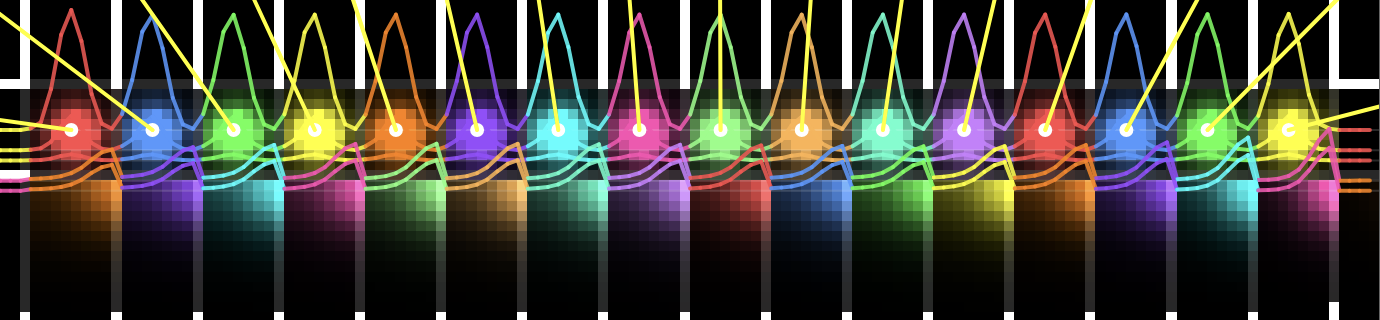
\includegraphics[width=\textwidth]{pictures/cable_domains.png}
\caption{The cable, relaxed. Sixteen sites along the axis, each with a kernel of charge $+3$, a core
domain of two electrons confined within $2.4\,a_0$, and one valence electron outside it. Colour
distinguishes domains; white verticals mark the free boundaries between neighbouring carriers, the
coloured curves are density profiles along the axis, and the yellow segments are net forces on the
kernels. Every boundary shown is an unknown of the minimisation.}
\label{fig:cable-domains}
\end{figure}

\paragraph{What sets the pinning.}
The barrier is set less by the strength of the ion lattice than by whether the carriers bunch into
its wells: a carrier distribution that resisted being modulated would ride over the lattice, one
that does not resist locks to it. RealQM's free interface resists very little, and this is internal
to the construction --- a flat density is admissible on a free boundary at no cost, so redrawing an
interface between domains of equal density is free, and the only penalty on a \emph{modulated}
density is the gradient term, carrying the coefficient $\tfrac12$.

That coefficient is a standardisation, not a constant of the theory: it is set by calibrating
against atomic spectra, on a bound electron in a single potential well. An extended arrangement is a
different object, and the coefficient governing how a carrier lattice resists modulation by an ion
lattice has no obligation to equal the one an atom's spectrum sets. So the natural thing is to ask
how much the answer turns on it. Doubling it --- a round factor, chosen for being round, not
calibrated to reproduce anything --- and leaving ions, standoff, geometry and mesh unchanged gives
$\varepsilon_{\rm bulk}\approx24$~meV, an elevenfold fall, to thermal energy at room temperature.

A barrier at $kT$ does not confine, so the pinning no longer holds and the charge is free to move.
What state the system is then in this measurement does not determine. It is not \emph{band}
conduction, since non-overlap admits no extended states for a band to be made of --- but that rules
out a mechanism, not a phenomenon, and whether the unpinned state would behave as a metal, as a
sliding charge lattice, or as something else is a question the instrument cannot reach. The
instrument measures a barrier; when the barrier goes, so does the instrument.

\paragraph{From a barrier to a conductivity.}
In the activated regime the corrugation is the activation energy in
$\sigma=(ne^2a^2\nu/kT)\,e^{-E_a/kT}$, where the exponential is the fraction of the time the system
is over the barrier and the prefactor $\nu=(1/2\pi)\sqrt{K/M}$ is how often it asks --- the
small-oscillation frequency of the collective coordinate, the charge pattern rocking against the ion
lattice. Since it is the sites that move, that rocking is a lattice vibration and $M$ is an ionic
mass. With $M=28\,u$ at $300$~K the two activated arrangements give $2\times10^{-12}$ and
$6.5$~S\,m$^{-1}$ --- glass and intrinsic germanium --- and the attempt frequencies come out at
$10^{12}$--$10^{13}$~Hz, the middle one at $11$~meV or $90$~cm$^{-1}$, an ordinary low-lying phonon.
Nothing was arranged to make that so, and it is the check that the mass entering $\nu$ is the right
kind of mass.

Three things enter from outside and should be named. The curvature $K$ is taken from an assumed
sinusoidal shape, since only the endpoints of $E(d)$ were computed. The mass is imported, because
RealQM carries no masses --- the coefficient of $|\nabla\psi_i|^2$ is a geometric scale, not
$\hbar^2/2m$, which is exactly why it could be doubled above. And $n=1/a^3$ is a convention for
turning a per-carrier barrier on a line of sites into a bulk conductivity. What the framework
supplies is the exponent.

\paragraph{Status.}
These barriers are rigid-slide values --- all carriers displaced together --- and that is the
expensive path. The cheap one is a kink: one carrier advancing while the rest hold still,
compressing the domains ahead and expanding those behind, at a cost independent of chain length.
Real conductors use kinks, so every barrier here is an upper bound and every conductivity a lower
bound, by a factor not yet determined. The carriers-on-a-substrate system is a Frenkel--Kontorova
chain, and in that reading the kink has its own width and its own limiting velocity, both computable
from two curvatures of the energy; neither is measured yet. Nor is the mesh convergence of the
$240$~meV, which is the first thing a reader should ask for and which is under test at the time of
writing. The instrument, at least, is sound: junction cancellation is exact by construction,
linearity is tested against a third window, translation by one spacing must return the same energy
to the last digit, and domains related by a symmetry must have equal eigenvalues.

\section{Roadmap toward broader materials applications}\label{sec:material-roadmap}

The validated materials-science regime of Chapter~\ref{ch:condensed} (ionic crystals, molecular crystals where electrostatics dominates) is the working bottom of a larger ambition. We sketch what extensions would enable the framework to reach further into the materials-science landscape.

\paragraph{Metals.}
Metallic bonding is delocalised: conduction electrons spread across many atoms, and the non-overlapping unit-density picture of Level 3 has to be extended to accommodate this. This has now been examined directly rather than left as a prospect, and the outcome is that the extension is not optional but structural.

Section~\ref{sec:conduction} puts this to the test directly, and the outcome is more interesting than
a flat exclusion. A chain of one-valence-electron atoms does behave as a dielectric: each domain
carries exactly one electron by constraint, so no charge passes between sites and the polarisability
is extensive before anything is computed --- confirmed as $\alpha=27.4N$, flat to $1\%$ per atom.
But rearranging the same charge into a cable of ions surrounded by carriers drops the barrier into
the semiconductor range, and stiffening the carriers removes it altogether.

Underneath the arithmetic one obstacle is genuinely structural: non-overlap makes the transfer
integral vanish identically. The transfer integral \emph{is} the overlap of neighbouring orbitals,
and there is none --- so the construction is not the Mott limit ($U\to\infty$ with $t\neq0$,
insulating but alive, conducting when doped) but the \emph{atomic limit}, where doping activates
nothing. \emph{Band} conduction is therefore absent in kind and not by degree: there are no extended
states for a band to be made of. That is a statement about a mechanism, and it does not by itself
decide whether the framework can produce conducting behaviour by another route --- which is the open
question Section~\ref{sec:conduction} ends on. A relaxed constraint permitting overlapping valence
territories would change the postulate rather than refine the implementation, and is one way out;
whether it is the only one is not established.

\paragraph{Semiconductors.}
Semiconductor physics as usually formulated depends on a small band gap and on the response of that gap to dopants, strain, and external fields --- and a band gap is a property of a band structure, which for the reason just given the Level-3 construction does not possess. That route is closed. Geometry the framework does reach: the tetrahedral and zincblende bonding topologies of Si, Ge and GaAs are within the angular splitting of the kernel valence sector, and cohesion, elastic response and defect energetics follow from it. And the \emph{transport} of the activated conductors turns out to be reachable by a different road, without a gap: Section~\ref{sec:conduction} measures a hopping barrier of ${\approx}240$~meV for a cable of ions, which is the activation energy such materials are characterised by. What remains outside is everything specifically tied to promotion across a gap --- intrinsic carrier statistics, the doping response through $t$, optical absorption edges.

\paragraph{Polymers and soft matter.}
Polymer chains and soft-matter systems are at the boundary between the molecular and the condensed regimes covered in Chapters~\ref{ch:folding} and~\ref{ch:condensed}. The Level-5 residue-level reduction of Chapter~\ref{ch:hierarchy} extends naturally to polymer monomer-level reductions, treating each monomer as an effective unit with appropriate electrostatic and steric profile.

\paragraph{Biological materials.}
Bones, shells, membranes, structural proteins (collagen, keratin), and biomineralisation are biological materials whose mechanical and electrostatic properties emerge from the interplay of atomic-scale interactions and supramolecular organisation. The hierarchy of Chapter~\ref{ch:hierarchy} reaches from atoms (Level 1) through proteins (Level 5) toward cellular structures (Level 6); biological materials lie in the Level-5 to Level-6 range, and the framework's reach into this regime is part of the vision Chapter~\ref{ch:hierarchy} sets out.

\paragraph{Electrochemistry and catalysis.}
Reactions at metal--solution interfaces (fuel cells, batteries, heterogeneous catalysis) are materials-science problems with an explicit chemistry component. RealQM's reactive chemistry handling (Chapter~\ref{ch:dimers}) combined with its Brownian-dynamics machinery (Chapter~\ref{ch:condensed}) puts the framework in a position to address such systems once the metal-extension above is in place.

\section{The framework's place in computational materials science}\label{sec:material-place}

We do not claim that RealQM is a replacement for DFT-MD or for empirical force fields in the materials-science workflow that has developed since the 1980s. Each tool has its regime; each tool has accuracy at a price the others do not pay.

\paragraph{What DFT-MD does that RealQM does not.}
\begin{itemize}
\item Chemical accuracy on covalent solids (silicon, diamond, transition-metal oxides) at well-validated functional level.
\item Band-structure and optical-property calculations through GW, BSE, and TD-DFT.
\item Dispersion correction (DFT-D3, MBD) at the post-DFT level for layered materials, molecular crystals, and biomolecules.
\item Decades of validated workflow: ground-state geometry, vibrational frequencies, elastic constants, thermal conductivity.
\end{itemize}

\paragraph{What empirical force fields do that RealQM does not.}
\begin{itemize}
\item Multi-microsecond molecular dynamics on protein-scale systems with known parameter sets.
\item Coarse-grained models (MARTINI, etc.) that reach mesoscale at low cost.
\item Reactive force fields (ReaxFF, REBO) for bond-breaking dynamics at scale.
\end{itemize}

\paragraph{What RealQM does that the others do not.}
\begin{itemize}
\item Ab initio condensed-phase phase transitions with no fitted parameters, at interactive cost on consumer hardware.
\item A unified framework that handles atoms, molecules, reactions, folding, and condensed phases from the same equation.
\item A regime-of-validity diagnostic (overshoot vs.\ missing dispersion) that the framework reports itself.
\item Interactive browser-based simulations suitable for pedagogy and rapid hypothesis exploration.
\item Real-space wave functions visualisable as charge densities, in continuity with Schr\"odinger's 1926 picture.
\end{itemize}

The framework's contribution to computational materials science is therefore complementary to the existing tools rather than competitive with them. It opens regimes that have been impractical (interactive condensed-phase exploration, real-time parameter sweeps on small materials systems) while leaving high-precision regimes to the established workflows.

\section{Significance: materials from a single principle}\label{sec:material-significance}

The most important statement of the materials chapter is structural rather than quantitative: \textbf{the same multiphase 3D continuum equation that handles a hydrogen atom (Chapter~\ref{ch:atoms}) handles a sodium-chloride crystal at finite temperature (Chapter~\ref{ch:condensed}), a protein folding under quantum-mechanical H-bond forces (Chapter~\ref{ch:folding}), and the helium-4 nucleus (Chapter~\ref{ch:nucleus}).} Materials science is, on this view, one application of a single variational principle that runs from femtometers to nanometers.

The accuracy of any one application varies with the regime --- chemistry at 1--10\%, condensed phases with calibrated overshoot, nuclear physics still exploratory --- but the underlying object is one equation. This is what is meant when the article and this book talk about the framework reaching scales beyond chemistry. Materials science is one of those scales; the rest of Part~III has worked through the others.

The next chapter takes the framework to Level 0 of the hierarchy, where the constituents are protons and electrons instead of electrons-around-a-kernel, and reports the validation of the same equation at the nuclear scale.

% --- End of Materials chapter ---
